% Options for packages loaded elsewhere
\PassOptionsToPackage{unicode}{hyperref}
\PassOptionsToPackage{hyphens}{url}
%
\documentclass[
]{article}
\usepackage{amsmath,amssymb}
\usepackage{iftex}
\ifPDFTeX
  \usepackage[T1]{fontenc}
  \usepackage[utf8]{inputenc}
  \usepackage{textcomp} % provide euro and other symbols
\else % if luatex or xetex
  \usepackage{unicode-math} % this also loads fontspec
  \defaultfontfeatures{Scale=MatchLowercase}
  \defaultfontfeatures[\rmfamily]{Ligatures=TeX,Scale=1}
\fi
\usepackage{lmodern}
\ifPDFTeX\else
  % xetex/luatex font selection
\fi
% Use upquote if available, for straight quotes in verbatim environments
\IfFileExists{upquote.sty}{\usepackage{upquote}}{}
\IfFileExists{microtype.sty}{% use microtype if available
  \usepackage[]{microtype}
  \UseMicrotypeSet[protrusion]{basicmath} % disable protrusion for tt fonts
}{}
\makeatletter
\@ifundefined{KOMAClassName}{% if non-KOMA class
  \IfFileExists{parskip.sty}{%
    \usepackage{parskip}
  }{% else
    \setlength{\parindent}{0pt}
    \setlength{\parskip}{6pt plus 2pt minus 1pt}}
}{% if KOMA class
  \KOMAoptions{parskip=half}}
\makeatother
\usepackage{xcolor}
\usepackage[margin=1in]{geometry}
\usepackage{graphicx}
\makeatletter
\newsavebox\pandoc@box
\newcommand*\pandocbounded[1]{% scales image to fit in text height/width
  \sbox\pandoc@box{#1}%
  \Gscale@div\@tempa{\textheight}{\dimexpr\ht\pandoc@box+\dp\pandoc@box\relax}%
  \Gscale@div\@tempb{\linewidth}{\wd\pandoc@box}%
  \ifdim\@tempb\p@<\@tempa\p@\let\@tempa\@tempb\fi% select the smaller of both
  \ifdim\@tempa\p@<\p@\scalebox{\@tempa}{\usebox\pandoc@box}%
  \else\usebox{\pandoc@box}%
  \fi%
}
% Set default figure placement to htbp
\def\fps@figure{htbp}
\makeatother
\setlength{\emergencystretch}{3em} % prevent overfull lines
\providecommand{\tightlist}{%
  \setlength{\itemsep}{0pt}\setlength{\parskip}{0pt}}
\setcounter{secnumdepth}{5}
\usepackage{booktabs}
\usepackage{longtable}
\usepackage{array}
\usepackage{multirow}
\usepackage{wrapfig}
\usepackage{float}
\usepackage{colortbl}
\usepackage{pdflscape}
\usepackage{tabu}
\usepackage{threeparttable}
\usepackage{threeparttablex}
\usepackage[normalem]{ulem}
\usepackage{makecell}
\usepackage{xcolor}
\usepackage[]{natbib}
\bibliographystyle{plainnat}
\usepackage{bookmark}
\IfFileExists{xurl.sty}{\usepackage{xurl}}{} % add URL line breaks if available
\urlstyle{same}
\hypersetup{
  pdftitle={Phantom-Words with simultaneous visual presentation - Results},
  pdfkeywords={Keywords},
  hidelinks,
  pdfcreator={LaTeX via pandoc}}

\title{Phantom-Words with simultaneous visual presentation - Results}
\author{Ansgar D. Endress\\
City, University of London}
\date{}

\begin{document}
\maketitle
\begin{abstract}
Abstract (to be written)
\end{abstract}

\section{Predictions}\label{predictions}

The predictions for the current experiment were unclear. On the one
hand, it is plausible that observers might encode entire scenes when
they are presented simultaneously. If so, they should not accept
phantom-words. On the other hand, statistical learning might operate
similarly for simultaneous as for sequential presentation. If so, the
results with sequential presentations should be replicated, especially
because the shapes appear as distinct individual shapes rather than
wholes. Further, presenting the shapes as whole in an object (i.e., in
the white on black presentation) might encourage observers to process
the combination of shapes as a single hole, leading to the rejection of
phantom words.

\section{Analysis}\label{analysis}

\subsection{Demographics}\label{demographics}

The main experiment recruited participants from testable minds
(\url{https://minds.testable.org/}). A pilot experiment recruited
participants from first year students at City, University of London
(UK). In the latter population, other experiments typically need to
exclude 30\% to 50\% of the sample due to insufficient attention.
Unfortunately, the present experiment does not offer a clear
performance-based criterion to make sure that participants paid
attention to the stimuli, as the task might be genuinely difficult.
However, given that my main interest lies in the performance on trials
involving phantom-words for participants who succeeded in the
statistical learning task, it is more conservative to exclude
participants whom might not have paid attention to the task, even if
this overestimates the statistical learning abilities.

As a result, I rely on the assumption that earlier statistical learning
literature has shown that participants can learn statistical relations
\emph{in principle}, and exclude those participants not exceeding an
accuracy of 50\% on word vs.~part-word trials. This criterion led to the
removal of 23 and 53 participants from the students and testable
samples, respectively. I present the results from these restricted
samples jointly with the results from the full sample. The demographics
of the full sample as well as the restricted sample are given in Table
\ref{tab:vsl-simultaneous-fa-demographics}. In the student sample, age
and gender were not recorded due to experimenter error.

\subsection{Analysis strategy}\label{analysis-strategy}

I will analyze the results using two types of analyses. First, I compare
the performance in the different trial types to the chance level of 50\%
using Wilcoxon tests. To compare performance across trial types, I
calculate normalized difference scores, that is,
\(\frac{\text{accuracy}_{\text{trial type 1}} - \text{accuracy}_{\text{trial type 2}}}{\text{accuracy}_{\text{trial type 1}} + \text{accuracy}_{\text{trial type 2}}}\).
These difference scores are the compared to the chance level of zero,
again using Wilcoxon tests. I also ask whether any of these results is
affected by the color polarity type (i.e., black on white vs.~white on
black). Following \citep{Rosenthal1999}, I use these focused analyses to
target the contrasts of interest, and so that the visualizations match
the statistical tests.

Second, I will confirm these results using a set of generalized linear
mixed models with the fixed factor predictors trial type and and color
polarity as well as their interaction, and a random intercept for
participants. I fitted separate model for each (full vs.~restricted)
sample and trial contrast (word vs.~part-word trials vs.~word
vs.~phantom-word trials and word vs.~part-words and phantom-word
vs.~part-word trials).

Results from the much larger main sample will be presented in the main
text. Results from the student sample will be presented in Supplementary
Online Material XXX.

\begin{longtable}[t]{lllrrrrrl}
\caption{\label{tab:vsl-simultaneous-fa-demographics}Demographics of the full sample and the restricted sample, where participants were excluded whose accuracy on word vs. part-words trials did not exceed 50 percent. For the student population, age and gender have not been recorded due to experimenter error.}\\
\toprule
Population & Sample type & Color polarity & N & Females & Males & Other & Age & Age range\\
\midrule
testable & Full sample & black on white & 82 & 47 & 35 & 0 & 30.3 & 19-66\\
testable & Full sample & white on black & 79 & 33 & 46 & 0 & 30.5 & 18-57\\
students & Full sample & black on white & 23 & 0 & 0 & 23 &  & Inf--Inf\\
students & Full sample & white on black & 27 & 0 & 0 & 27 &  & Inf--Inf\\
testable & Restricted sample & black on white & 57 & 32 & 25 & 0 & 30.7 & 19-59\\
\addlinespace
testable & Restricted sample & white on black & 51 & 22 & 29 & 0 & 31.9 & 18-57\\
students & Restricted sample & black on white & 12 & 0 & 0 & 12 &  & Inf--Inf\\
students & Restricted sample & white on black & 15 & 0 & 0 & 15 &  & Inf--Inf\\
\bottomrule
\end{longtable}

\subsection{Analysis by accuracy}\label{analysis-by-accuracy}

\begin{longtable}[t]{lrrrrrr}
\caption{\label{tab:vsl-simultaneous-fa-descriptives-print-testable}Descriptives of accuracy scores and difference scores for the main sample. The restricted sample consists of participants whose performance exceeded 50\% on word vs. part-word trials. The p value reflects a Wilcoxon test against the chance levels of 50 percent and of zero for accuracies and difference scores, respectively. The effect of color polarity represents a Wilcoxon test comparing all of these dependent variables as a function of color polarity. The p value was corrected for repeated testing using the Holm-Bonferroni method, separately for each (full or restricted) sample (pHB). In the restricted sample, comparisons of the word vs. part-word contrast against chance are not meaningful as participants were selected based on their performance in this comparison.}\\
\toprule
test.type & M & SE & p.wilcox & p.hb & r.wilcox & power\\
\midrule
\endfirsthead
\caption[]{Descriptives of accuracy scores and difference scores for the main sample. The restricted sample consists of participants whose performance exceeded 50\% on word vs. part-word trials. The p value reflects a Wilcoxon test against the chance levels of 50 percent and of zero for accuracies and difference scores, respectively. The effect of color polarity represents a Wilcoxon test comparing all of these dependent variables as a function of color polarity. The p value was corrected for repeated testing using the Holm-Bonferroni method, separately for each (full or restricted) sample (pHB). In the restricted sample, comparisons of the word vs. part-word contrast against chance are not meaningful as participants were selected based on their performance in this comparison. \textit{(continued)}}\\
\toprule
test.type & M & SE & p.wilcox & p.hb & r.wilcox & power\\
\midrule
\endhead

\endfoot
\bottomrule
\endlastfoot
\addlinespace[0.3em]
\multicolumn{7}{l}{\textbf{Full sample - Zcombined (N = 161)}}\\
\cellcolor{gray!10}{\hspace{1em}w.pw} & \cellcolor{gray!10}{60.093} & \cellcolor{gray!10}{1.281} & \cellcolor{gray!10}{0.000} & \cellcolor{gray!10}{0.000} & \cellcolor{gray!10}{0.550} & \cellcolor{gray!10}{1.000}\\
\hspace{1em}w.phw & 48.292 & 1.158 & 0.571 & 1.000 & 0.045 & 0.313\\
\cellcolor{gray!10}{\hspace{1em}phw.pw} & \cellcolor{gray!10}{58.333} & \cellcolor{gray!10}{1.303} & \cellcolor{gray!10}{0.000} & \cellcolor{gray!10}{0.000} & \cellcolor{gray!10}{0.453} & \cellcolor{gray!10}{1.000}\\
\hspace{1em}d.relative.w.pw.w.phw & 0.111 & 0.016 & 0.000 & 0.000 & 0.488 & 1.000\\
\cellcolor{gray!10}{\hspace{1em}d.relative.w.pw.ph.pw} & \cellcolor{gray!10}{0.016} & \cellcolor{gray!10}{0.014} & \cellcolor{gray!10}{0.519} & \cellcolor{gray!10}{1.000} & \cellcolor{gray!10}{0.051} & \cellcolor{gray!10}{0.199}\\
\addlinespace[0.3em]
\multicolumn{7}{l}{\textbf{Full sample - black.on.white (N = 82)}}\\
\hspace{1em}w.pw & 60.671 & 1.795 & 0.000 & 0.000 & 0.550 & 1.000\\
\cellcolor{gray!10}{\hspace{1em}w.phw} & \cellcolor{gray!10}{47.764} & \cellcolor{gray!10}{1.633} & \cellcolor{gray!10}{0.495} & \cellcolor{gray!10}{1.000} & \cellcolor{gray!10}{0.075} & \cellcolor{gray!10}{0.275}\\
\hspace{1em}phw.pw & 56.606 & 1.738 & 0.000 & 0.005 & 0.387 & 0.965\\
\cellcolor{gray!10}{\hspace{1em}d.relative.w.pw.w.phw} & \cellcolor{gray!10}{0.120} & \cellcolor{gray!10}{0.022} & \cellcolor{gray!10}{0.000} & \cellcolor{gray!10}{0.000} & \cellcolor{gray!10}{0.509} & \cellcolor{gray!10}{1.000}\\
\hspace{1em}d.relative.w.pw.ph.pw & 0.034 & 0.019 & 0.147 & 1.000 & 0.160 & 0.428\\
\addlinespace[0.3em]
\multicolumn{7}{l}{\textbf{Full sample - white.on.black (N = 79)}}\\
\cellcolor{gray!10}{\hspace{1em}w.pw} & \cellcolor{gray!10}{59.494} & \cellcolor{gray!10}{1.849} & \cellcolor{gray!10}{0.000} & \cellcolor{gray!10}{0.000} & \cellcolor{gray!10}{0.548} & \cellcolor{gray!10}{0.999}\\
\hspace{1em}w.phw & 48.840 & 1.660 & 0.869 & 1.000 & 0.019 & 0.107\\
\cellcolor{gray!10}{\hspace{1em}phw.pw} & \cellcolor{gray!10}{60.127} & \cellcolor{gray!10}{1.951} & \cellcolor{gray!10}{0.000} & \cellcolor{gray!10}{0.000} & \cellcolor{gray!10}{0.517} & \cellcolor{gray!10}{0.999}\\
\hspace{1em}d.relative.w.pw.w.phw & 0.101 & 0.023 & 0.000 & 0.001 & 0.458 & 0.992\\
\cellcolor{gray!10}{\hspace{1em}d.relative.w.pw.ph.pw} & \cellcolor{gray!10}{-0.003} & \cellcolor{gray!10}{0.021} & \cellcolor{gray!10}{0.701} & \cellcolor{gray!10}{1.000} & \cellcolor{gray!10}{0.043} & \cellcolor{gray!10}{0.053}\\
\addlinespace[0.3em]
\multicolumn{7}{l}{\textbf{Full sample - zEffect of color polarity}}\\
\hspace{1em}w.pw &  &  & 0.607 & 1.000 & 0.041 & 0.074\\
\cellcolor{gray!10}{\hspace{1em}w.phw} & \cellcolor{gray!10}{} & \cellcolor{gray!10}{} & \cellcolor{gray!10}{0.458} & \cellcolor{gray!10}{1.000} & \cellcolor{gray!10}{0.058} & \cellcolor{gray!10}{0.075}\\
\hspace{1em}phw.pw &  &  & 0.227 & 1.000 & 0.095 & 0.272\\
\cellcolor{gray!10}{\hspace{1em}d.relative.w.pw.w.phw} & \cellcolor{gray!10}{} & \cellcolor{gray!10}{} & \cellcolor{gray!10}{0.519} & \cellcolor{gray!10}{1.000} & \cellcolor{gray!10}{0.051} & \cellcolor{gray!10}{0.088}\\
\hspace{1em}d.relative.w.pw.ph.pw &  &  & 0.263 & 1.000 & 0.088 & 0.262\\
\addlinespace[0.3em]
\multicolumn{7}{l}{\textbf{Restricted sample - Zcombined (N = 108)}}\\
\cellcolor{gray!10}{\hspace{1em}w.pw} & \cellcolor{gray!10}{69.136} & \cellcolor{gray!10}{1.011} & \cellcolor{gray!10}{0.000} & \cellcolor{gray!10}{0.000} & \cellcolor{gray!10}{0.876} & \cellcolor{gray!10}{1.000}\\
\hspace{1em}w.phw & 49.306 & 1.432 & 0.903 & 1.000 & 0.012 & 0.077\\
\cellcolor{gray!10}{\hspace{1em}phw.pw} & \cellcolor{gray!10}{60.957} & \cellcolor{gray!10}{1.587} & \cellcolor{gray!10}{0.000} & \cellcolor{gray!10}{0.000} & \cellcolor{gray!10}{0.556} & \cellcolor{gray!10}{1.000}\\
\hspace{1em}d.relative.w.pw.w.phw & 0.180 & 0.015 & 0.000 & 0.000 & 0.776 & 1.000\\
\cellcolor{gray!10}{\hspace{1em}d.relative.w.pw.ph.pw} & \cellcolor{gray!10}{0.075} & \cellcolor{gray!10}{0.015} & \cellcolor{gray!10}{0.000} & \cellcolor{gray!10}{0.000} & \cellcolor{gray!10}{0.419} & \cellcolor{gray!10}{0.999}\\
\addlinespace[0.3em]
\multicolumn{7}{l}{\textbf{Restricted sample - black.on.white (N = 57)}}\\
\hspace{1em}w.pw & 69.152 & 1.395 & 0.000 & 0.000 & 0.878 & 1.000\\
\cellcolor{gray!10}{\hspace{1em}w.phw} & \cellcolor{gray!10}{49.269} & \cellcolor{gray!10}{2.065} & \cellcolor{gray!10}{0.905} & \cellcolor{gray!10}{1.000} & \cellcolor{gray!10}{0.016} & \cellcolor{gray!10}{0.064}\\
\hspace{1em}phw.pw & 58.626 & 1.985 & 0.000 & 0.001 & 0.531 & 0.991\\
\cellcolor{gray!10}{\hspace{1em}d.relative.w.pw.w.phw} & \cellcolor{gray!10}{0.182} & \cellcolor{gray!10}{0.021} & \cellcolor{gray!10}{0.000} & \cellcolor{gray!10}{0.000} & \cellcolor{gray!10}{0.760} & \cellcolor{gray!10}{1.000}\\
\hspace{1em}d.relative.w.pw.ph.pw & 0.091 & 0.021 & 0.000 & 0.001 & 0.518 & 0.991\\
\addlinespace[0.3em]
\multicolumn{7}{l}{\textbf{Restricted sample - white.on.black (N = 51)}}\\
\cellcolor{gray!10}{\hspace{1em}w.pw} & \cellcolor{gray!10}{69.118} & \cellcolor{gray!10}{1.496} & \cellcolor{gray!10}{0.000} & \cellcolor{gray!10}{0.000} & \cellcolor{gray!10}{0.878} & \cellcolor{gray!10}{1.000}\\
\hspace{1em}w.phw & 49.346 & 2.012 & 0.985 & 1.000 & 0.003 & 0.062\\
\cellcolor{gray!10}{\hspace{1em}phw.pw} & \cellcolor{gray!10}{63.562} & \cellcolor{gray!10}{2.516} & \cellcolor{gray!10}{0.000} & \cellcolor{gray!10}{0.000} & \cellcolor{gray!10}{0.584} & \cellcolor{gray!10}{1.000}\\
\hspace{1em}d.relative.w.pw.w.phw & 0.178 & 0.021 & 0.000 & 0.000 & 0.797 & 1.000\\
\cellcolor{gray!10}{\hspace{1em}d.relative.w.pw.ph.pw} & \cellcolor{gray!10}{0.056} & \cellcolor{gray!10}{0.021} & \cellcolor{gray!10}{0.026} & \cellcolor{gray!10}{0.238} & \cellcolor{gray!10}{0.311} & \cellcolor{gray!10}{0.747}\\
\addlinespace[0.3em]
\multicolumn{7}{l}{\textbf{Restricted sample - zEffect of color polarity}}\\
\hspace{1em}w.pw &  &  & 0.959 & 1.000 & 0.005 & 0.050\\
\cellcolor{gray!10}{\hspace{1em}w.phw} & \cellcolor{gray!10}{} & \cellcolor{gray!10}{} & \cellcolor{gray!10}{0.878} & \cellcolor{gray!10}{1.000} & \cellcolor{gray!10}{0.015} & \cellcolor{gray!10}{0.050}\\
\hspace{1em}phw.pw &  &  & 0.125 & 1.000 & 0.148 & 0.343\\
\cellcolor{gray!10}{\hspace{1em}d.relative.w.pw.w.phw} & \cellcolor{gray!10}{} & \cellcolor{gray!10}{} & \cellcolor{gray!10}{0.784} & \cellcolor{gray!10}{1.000} & \cellcolor{gray!10}{0.026} & \cellcolor{gray!10}{0.052}\\
\hspace{1em}d.relative.w.pw.ph.pw &  &  & 0.331 & 1.000 & 0.094 & 0.218\\*
\end{longtable}

\begin{figure}

{\centering 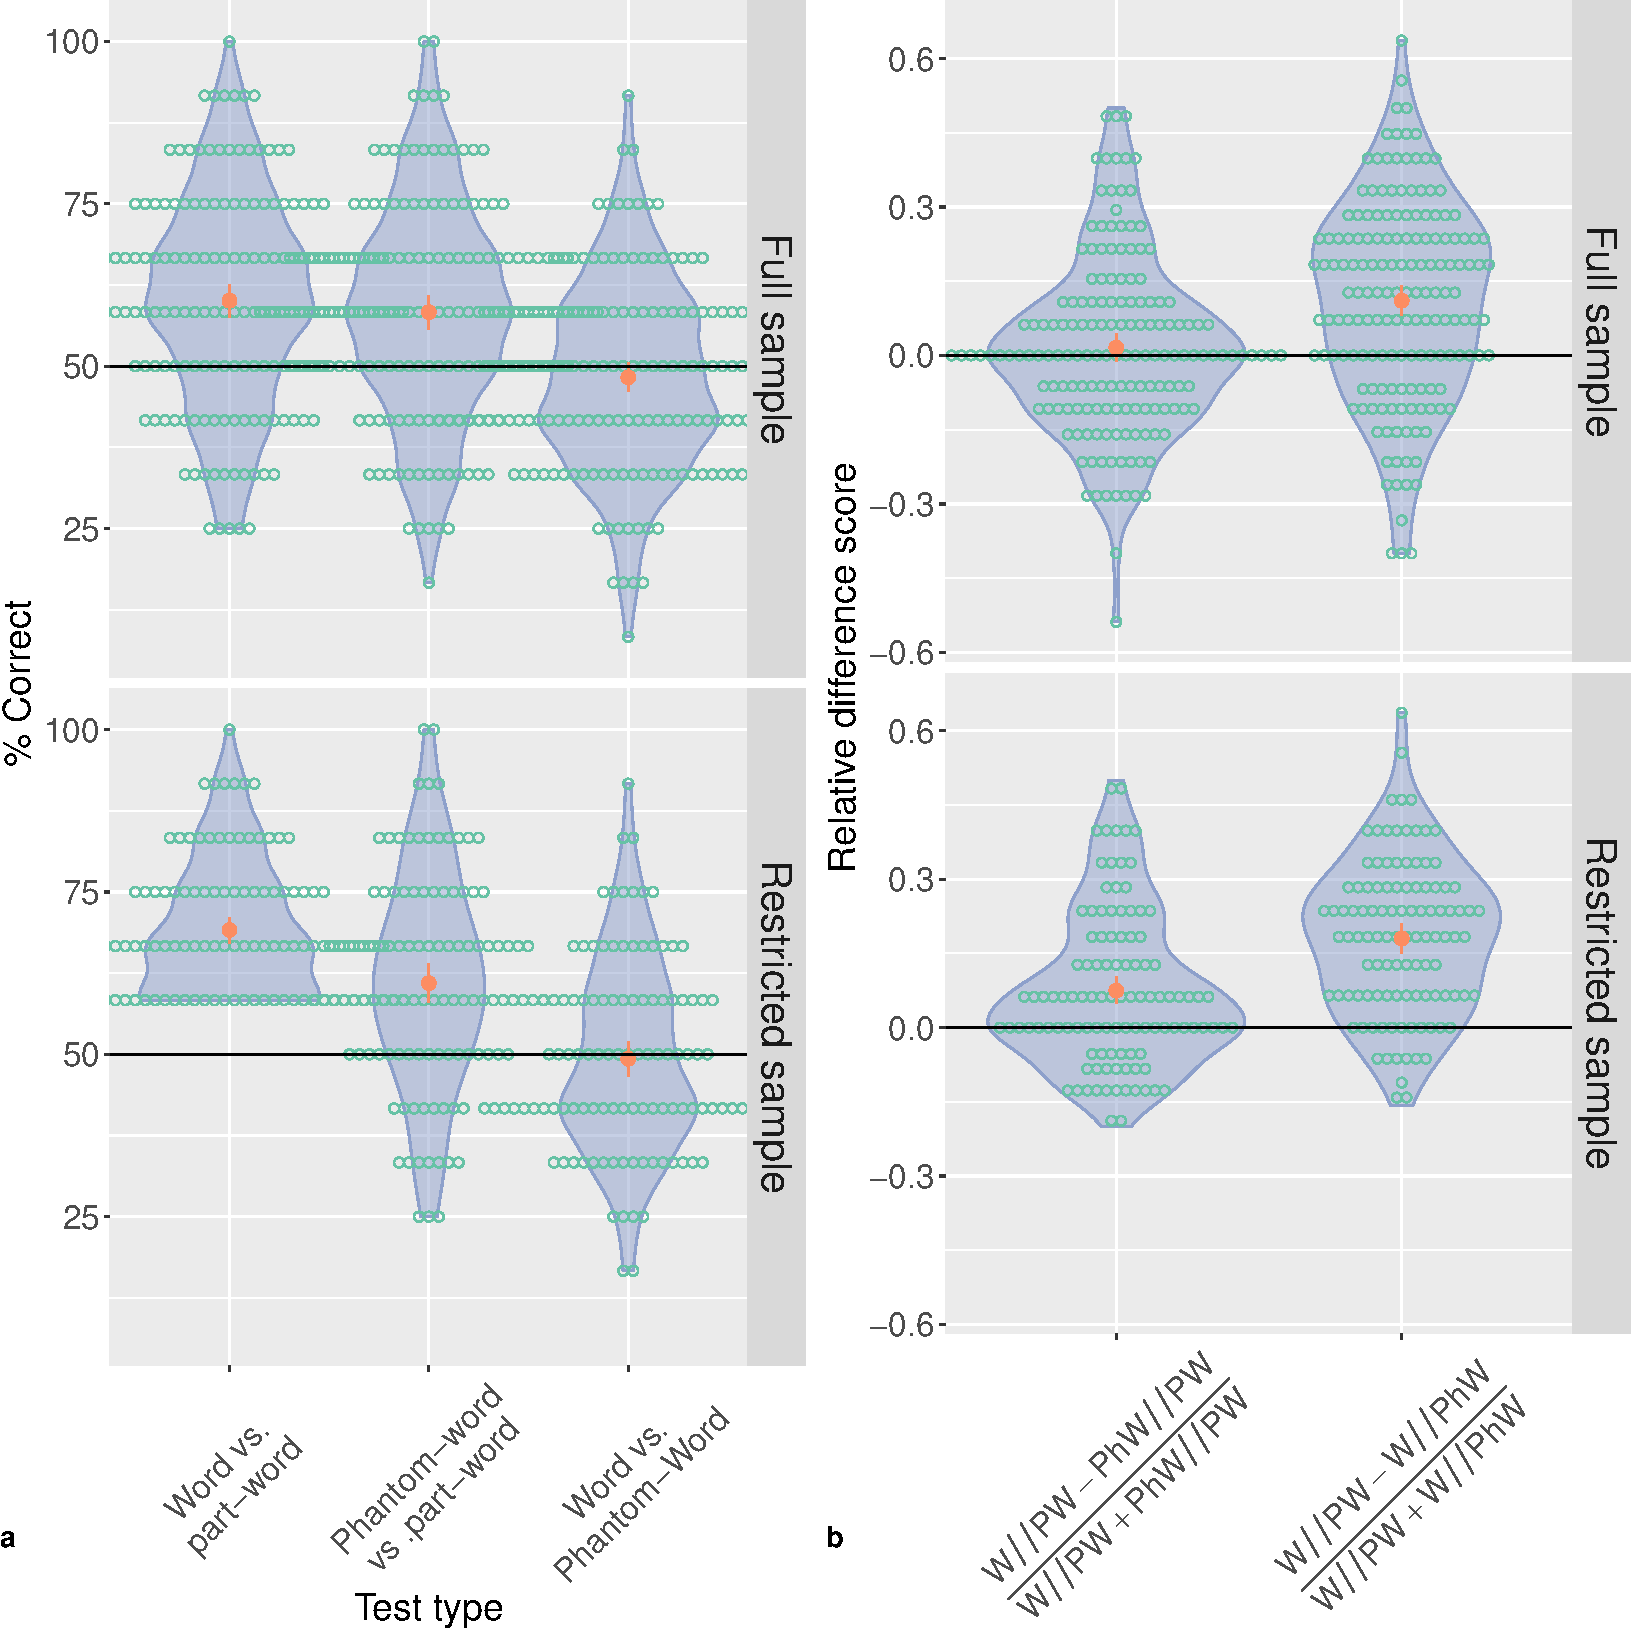
\includegraphics[width=0.8\linewidth]{vsl_phamtoms_simultaneous_results_files/figure-latex/vsl-simultaneous-fa-plot-accuracy-diff-scores-plot-polarity-collapsed-testable-1} 

}

\caption{(a) Accuracy in the different trial types (words vs. part-words, phantom-words vs. part-words, and words vs. phantom-words), (b)  Relative difference scores for contrasts between different trial types (word vs. part-word trials vs. phantom-word vs. part-word trials, and word vs. part-word trials vs. word vs. phantom-word trials). Both panels show the data for the full main sample (top) or after exclusion of participants whose performance did not exceed 50\% in the word vs. part-word trials (bottom), collapsed across polarity contrasts (black shapes on a white background vs. white shapes on a black background). The dots, error bars and violin represent the sample averages, 95\% bootstrap confidence intervals and the distribution of the average accuracy for individual participants, respectively. Empty circles represent individual participants.}\label{fig:vsl-simultaneous-fa-plot-accuracy-diff-scores-plot-polarity-collapsed-testable}
\end{figure}

As shown in Table
\ref{tab:vsl-simultaneous-fa-descriptives-print-testable} and Figure
\ref{fig:vsl-simultaneous-fa-plot-accuracy-diff-scores-plot-polarity-collapsed-testable}a,
participants from the main sample preferred both words and phantom-words
to part-words.\footnote{The above chance performance in the restricted
  sample is meaningless, since only those participants were included who
  exceeded 50\% on the word vs.~part-word test.} In contrast, they had
no preference for words over phantom-words. Similar results were
obtained for both color polarity types, with no discernible effect of
color polarity type. This results held in both the full sample and the
restricted sample. (Individual results for the different polarity types
are given in Figure
\ref{fig:vsl-simultaneous-fa-plot-accuracy-plot-by-polarity-testable}.)

To compare performance in the different trial types, I calculated the
difference scores mentioned above. As shown in Table
\ref{tab:vsl-simultaneous-fa-descriptives-print-testable} and Figure
\ref{fig:vsl-simultaneous-fa-plot-accuracy-diff-scores-plot-polarity-collapsed-testable}b,
participants from the testable sample performed much better on word
vs.~part-word trials than on word vs.~phantom-word trials, irrespective
of the color polarity type. This suggests that participants find
discriminations based on TPs much easier than discriminations based on
frequency of occurrence, which is problematic if statistical learning
leads to memory for units. (Individual results for the different
polarity types are given in Figure
\ref{fig:vsl-simultaneous-fa-plot-difference-scores-plot-testable}.)

However, at least in the restricted sample, performance was also
somewhat better for word vs.~part-word trials than for phantom-word
vs.~part-word trials, suggesting that we cannot rule out that
participants might also have some ability to track frequencies of
occurrence. However, the corresponding difference score was much smaller
than that comparing words vs.~part-word and word vs.~phantom-word
trials, and was not significant in the full sample.

As shown in Supplementary Online Material XXX, the results were similar
for the student samnple, except that the data was noisier.

\begin{longtable}[t]{lrrlrrlrrr}
\caption{\label{tab:vsl-simultaneous-fa-plot-glmer-correct-print-testable}Results of generalized linear mixed models for trial-by-trial responses, for the main sample. Results are reported for the full sample as well as the restricted sample, where participants were excluded if their performance did not exceed 50\% on the word vs. part-word trials.}\\
\toprule
\multicolumn{1}{c}{ } & \multicolumn{3}{c}{Log-odds} & \multicolumn{3}{c}{Odd ratios} & \multicolumn{2}{c}{ } & \multicolumn{2}{c}{Power} \\
\cmidrule(l{3pt}r{3pt}){2-4} \cmidrule(l{3pt}r{3pt}){5-7} \cmidrule(l{3pt}r{3pt}){10-11}
term & Estimate & SE & CI & Estimate & SE & CI & t & p & power\\
\midrule
\addlinespace[0.3em]
\multicolumn{10}{l}{\textbf{Full sample - w.pw vs. w.phw}}\\
\hspace{1em}test.typew.pw & 0.530 & 0.092 & {}[0.35, 0.711] & 1.700 & 0.156 & {}[1.42, 2.04] & 5.767 & 0.000 & 1.000\\
\hspace{1em}color.typewhite.on.black & 0.044 & 0.099 & {}[-0.151, 0.238] & 1.045 & 0.104 & {}[0.86, 1.27] & 0.440 & 0.660 & 0.069\\
\hspace{1em}test.typew.pw:color.typewhite.on.black & -0.093 & 0.131 & {}[-0.35, 0.163] & 0.911 & 0.119 & {}[0.705, 1.18] & -0.713 & 0.476 & 0.114\\
\addlinespace[0.3em]
\multicolumn{10}{l}{\textbf{Full sample - w.pw vs. phw.pw}}\\
\hspace{1em}test.typew.pw & 0.172 & 0.093 & {}[-0.00962, 0.355] & 1.188 & 0.110 & {}[0.99, 1.43] & 1.856 & 0.063 & 0.459\\
\hspace{1em}color.typewhite.on.black & 0.151 & 0.109 & {}[-0.0625, 0.364] & 1.162 & 0.126 & {}[0.939, 1.44] & 1.385 & 0.166 & 0.293\\
\hspace{1em}test.typew.pw:color.typewhite.on.black & -0.200 & 0.133 & {}[-0.46, 0.0609] & 0.819 & 0.109 & {}[0.631, 1.06] & -1.502 & 0.133 & 0.304\\
\addlinespace[0.3em]
\multicolumn{10}{l}{\textbf{Restricted sample - w.pw vs. w.phw}}\\
\hspace{1em}test.typew.pw & 0.836 & 0.113 & {}[0.616, 1.06] & 2.308 & 0.260 & {}[1.85, 2.88] & 7.422 & 0.000 & 1.000\\
\hspace{1em}color.typewhite.on.black & 0.003 & 0.111 & {}[-0.215, 0.221] & 1.003 & 0.112 & {}[0.807, 1.25] & 0.028 & 0.978 & 0.051\\
\hspace{1em}test.typew.pw:color.typewhite.on.black & -0.005 & 0.164 & {}[-0.326, 0.317] & 0.995 & 0.163 & {}[0.722, 1.37] & -0.029 & 0.977 & 0.058\\
\addlinespace[0.3em]
\multicolumn{10}{l}{\textbf{Restricted sample - w.pw vs. phw.pw}}\\
\hspace{1em}test.typew.pw & 0.460 & 0.114 & {}[0.237, 0.683] & 1.584 & 0.180 & {}[1.27, 1.98] & 4.047 & 0.000 & 0.981\\
\hspace{1em}color.typewhite.on.black & 0.209 & 0.117 & {}[-0.02, 0.437] & 1.232 & 0.144 & {}[0.98, 1.55] & 1.788 & 0.074 & 0.451\\
\hspace{1em}test.typew.pw:color.typewhite.on.black & -0.210 & 0.166 & {}[-0.536, 0.116] & 0.810 & 0.135 & {}[0.585, 1.12] & -1.263 & 0.207 & 0.249\\
\bottomrule
\end{longtable}

I confirmed these results using the generalized linear mixed models
mentioned above. As shown in Table
\ref{tab:vsl-simultaneous-fa-plot-glmer-correct-print-testable}, the
models showed that performance on word vs.~part-word trials was
significantly better than for word vs.~phantom-word trials. They also
showed that performance on word vs.~part-word trials was significantly
better than on phantom-word vs.~part-word trials, though this predictor
was significant only in the restricted sample and was only marginal in
the full sample. Further, the odds ratio associated with the former
contrast was almost twice as large as that from the latter contrast.

There were no main effects or interactions with polarity type. The
results for the student sample were generally similar.

\section{Discussion}\label{discussion}

\clearpage

\section{Appendix 1: Results split by polarity
type}\label{appendix-1-results-split-by-polarity-type}

\begin{figure}

{\centering 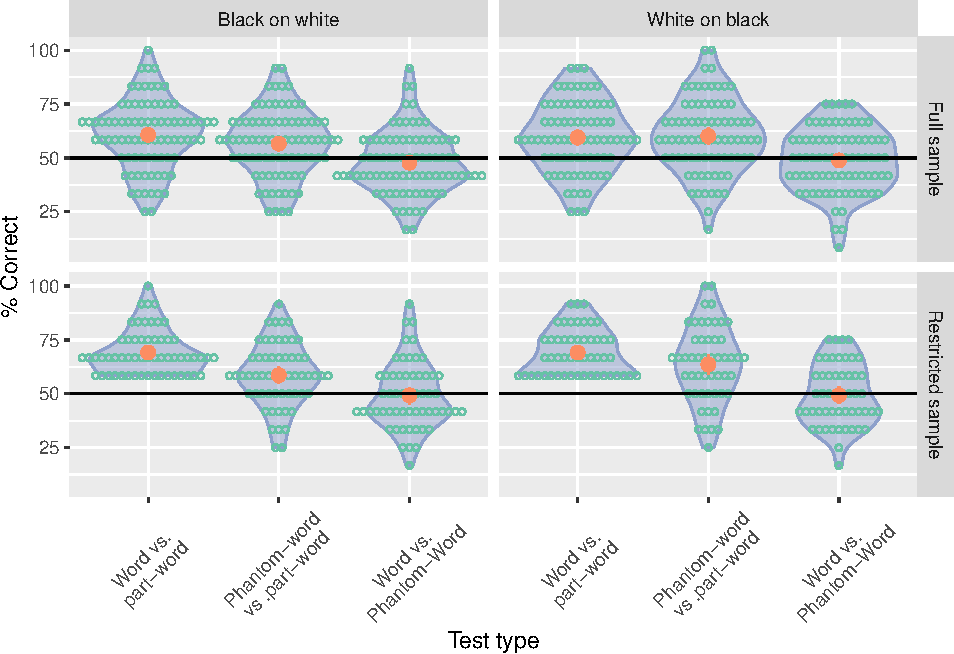
\includegraphics[width=0.8\linewidth]{vsl_phamtoms_simultaneous_results_files/figure-latex/vsl-simultaneous-fa-plot-accuracy-plot-by-polarity-testable-1} 

}

\caption{Accuracy in the different trial types (words vs. part-words, phantom-words vs. part-words, and words vs. phantom-words), for the full main sample (top) or after exclusion of participants whose performance did not exceed 50\% in the word vs. part-word trials (bottom), for black shapes on a white background (left) and white shapes on a black background (right). The dots, error bars and violin represent the sample averages, 95\% bootstrap confidence intervals and the distribution of the average accuracy for individual participants, respectively. Empty circles represent individual participants.}\label{fig:vsl-simultaneous-fa-plot-accuracy-plot-by-polarity-testable}
\end{figure}

\begin{figure}

{\centering 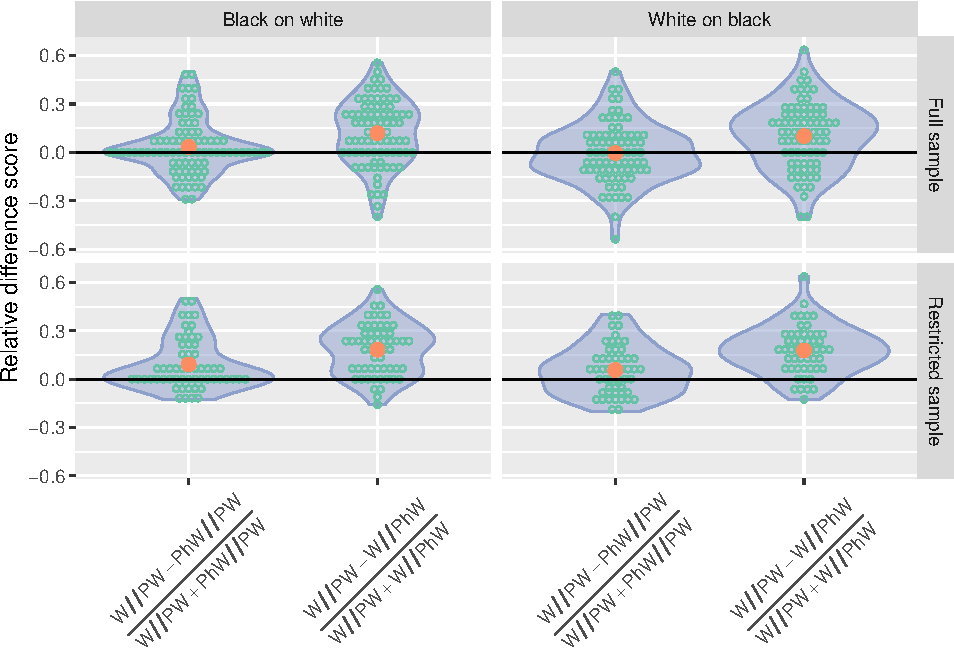
\includegraphics[width=0.8\linewidth]{vsl_phamtoms_simultaneous_results_files/figure-latex/vsl-simultaneous-fa-plot-difference-scores-plot-testable-1} 

}

\caption{Relative difference scores for contrasts between different trial types (word vs. part-word trials vs. phantom-word vs. part-word trials, and word vs. part-word trials vs. word vs. phantom-word trials), for the full main sample or after exclusion of participants whose performance did not exceed 50\% in the word vs. part-word trials. The dots, error bars and violin represent the sample averages, 95\% bootstrap confidence intervals and the distribution of the difference scores for individual participants, respectively. Empty circles represent individual participants.}\label{fig:vsl-simultaneous-fa-plot-difference-scores-plot-testable}
\end{figure}

\clearpage

\section{Appendix 2: Results with the student
sample}\label{appendix-2-results-with-the-student-sample}

\begin{longtable}[t]{lrrrrrr}
\caption{\label{tab:vsl-simultaneous-fa-descriptives-print-city}Descriptives of accuracy scores and difference scores for the student sample. The restricted sample consists of participants whose performance exceeded 50\% on word vs. part-word trials. The p value reflects a Wilcoxon test against the chance levels of 50 percent and of zero for accuracies and difference scores, respectively. The effect of color polarity represents a Wilcoxon test comparing all of these dependent variables as a function of color polarity. The p value was corrected for repeated testing using the Holm-Bonferroni method, separately for each (full or restricted) sample (pHB). In the restricted sample, comparisons of the word vs. part-word contrast against chance are not meaningful as participants were selected based on their performance in this comparison.}\\
\toprule
test.type & M & SE & p.wilcox & p.hb & r.wilcox & power\\
\midrule
\addlinespace[0.3em]
\multicolumn{7}{l}{\textbf{Full sample - Zcombined (N = 50)}}\\
\hspace{1em}w.pw & 56.167 & 2.066 & 0.009 & 0.163 & 0.369 & 0.840\\
\hspace{1em}w.phw & 46.833 & 2.392 & 0.163 & 1.000 & 0.197 & 0.259\\
\hspace{1em}phw.pw & 52.500 & 2.272 & 0.204 & 1.000 & 0.180 & 0.193\\
\hspace{1em}d.relative.w.pw.w.phw & 0.099 & 0.030 & 0.002 & 0.042 & 0.435 & 0.912\\
\hspace{1em}d.relative.w.pw.ph.pw & 0.038 & 0.026 & 0.165 & 1.000 & 0.196 & 0.300\\
\addlinespace[0.3em]
\multicolumn{7}{l}{\textbf{Full sample - black.on.white (N = 23)}}\\
\hspace{1em}w.pw & 57.246 & 2.695 & 0.012 & 0.196 & 0.527 & 0.748\\
\hspace{1em}w.phw & 45.652 & 3.706 & 0.182 & 1.000 & 0.278 & 0.209\\
\hspace{1em}phw.pw & 51.087 & 3.874 & 0.793 & 1.000 & 0.055 & 0.059\\
\hspace{1em}d.relative.w.pw.w.phw & 0.131 & 0.039 & 0.004 & 0.070 & 0.606 & 0.909\\
\hspace{1em}d.relative.w.pw.ph.pw & 0.071 & 0.043 & 0.130 & 1.000 & 0.316 & 0.372\\
\addlinespace[0.3em]
\multicolumn{7}{l}{\textbf{Full sample - white.on.black (N = 27)}}\\
\hspace{1em}w.pw & 55.247 & 3.145 & 0.196 & 1.000 & 0.249 & 0.374\\
\hspace{1em}w.phw & 47.840 & 3.224 & 0.601 & 1.000 & 0.101 & 0.101\\
\hspace{1em}phw.pw & 53.704 & 2.732 & 0.146 & 1.000 & 0.280 & 0.265\\
\hspace{1em}d.relative.w.pw.w.phw & 0.072 & 0.045 & 0.135 & 1.000 & 0.288 & 0.356\\
\hspace{1em}d.relative.w.pw.ph.pw & 0.009 & 0.032 & 0.716 & 1.000 & 0.070 & 0.059\\
\addlinespace[0.3em]
\multicolumn{7}{l}{\textbf{Full sample - zEffect of color polarity}}\\
\hspace{1em}w.pw &  &  & 0.781 & 1.000 & 0.039 & 0.076\\
\hspace{1em}w.phw &  &  & 0.553 & 1.000 & 0.084 & 0.073\\
\hspace{1em}phw.pw &  &  & 0.392 & 1.000 & 0.121 & 0.087\\
\hspace{1em}d.relative.w.pw.w.phw &  &  & 0.329 & 1.000 & 0.138 & 0.163\\
\hspace{1em}d.relative.w.pw.ph.pw &  &  & 0.250 & 1.000 & 0.163 & 0.220\\
\addlinespace[0.3em]
\multicolumn{7}{l}{\textbf{Restricted sample - Zcombined (N = 27)}}\\
\hspace{1em}w.pw & 66.975 & 1.601 & 0.000 & 0.000 & 0.883 & 1.000\\
\hspace{1em}w.phw & 51.543 & 3.683 & 0.602 & 1.000 & 0.100 & 0.070\\
\hspace{1em}phw.pw & 54.938 & 2.410 & 0.019 & 0.203 & 0.452 & 0.520\\
\hspace{1em}d.relative.w.pw.w.phw & 0.154 & 0.038 & 0.001 & 0.014 & 0.647 & 0.979\\
\hspace{1em}d.relative.w.pw.ph.pw & 0.106 & 0.028 & 0.001 & 0.016 & 0.638 & 0.963\\
\addlinespace[0.3em]
\multicolumn{7}{l}{\textbf{Restricted sample - black.on.white (N = 12)}}\\
\hspace{1em}w.pw & 67.361 & 2.262 & 0.002 & 0.032 & 0.885 & 1.000\\
\hspace{1em}w.phw & 52.778 & 5.392 & 0.623 & 1.000 & 0.142 & 0.078\\
\hspace{1em}phw.pw & 47.917 & 4.167 & 0.765 & 1.000 & 0.086 & 0.077\\
\hspace{1em}d.relative.w.pw.w.phw & 0.141 & 0.051 & 0.019 & 0.203 & 0.679 & 0.750\\
\hspace{1em}d.relative.w.pw.ph.pw & 0.180 & 0.045 & 0.004 & 0.051 & 0.839 & 0.968\\
\addlinespace[0.3em]
\multicolumn{7}{l}{\textbf{Restricted sample - white.on.black (N = 15)}}\\
\hspace{1em}w.pw & 66.667 & 2.381 & 0.001 & 0.012 & 0.883 & 1.000\\
\hspace{1em}w.phw & 50.556 & 5.355 & 0.875 & 1.000 & 0.041 & 0.051\\
\hspace{1em}phw.pw & 60.556 & 1.968 & 0.002 & 0.032 & 0.797 & 0.999\\
\hspace{1em}d.relative.w.pw.w.phw & 0.165 & 0.058 & 0.018 & 0.203 & 0.608 & 0.784\\
\hspace{1em}d.relative.w.pw.ph.pw & 0.047 & 0.029 & 0.143 & 1.000 & 0.378 & 0.355\\
\addlinespace[0.3em]
\multicolumn{7}{l}{\textbf{Restricted sample - zEffect of color polarity}}\\
\hspace{1em}w.pw &  &  & 0.698 & 1.000 & 0.075 & 0.055\\
\hspace{1em}w.phw &  &  & 0.825 & 1.000 & 0.043 & 0.060\\
\hspace{1em}phw.pw &  &  & 0.008 & 0.107 & 0.508 & 0.834\\
\hspace{1em}d.relative.w.pw.w.phw &  &  & 0.807 & 1.000 & 0.047 & 0.061\\
\hspace{1em}d.relative.w.pw.ph.pw &  &  & 0.011 & 0.130 & 0.491 & 0.738\\
\bottomrule
\end{longtable}

\begin{figure}

{\centering 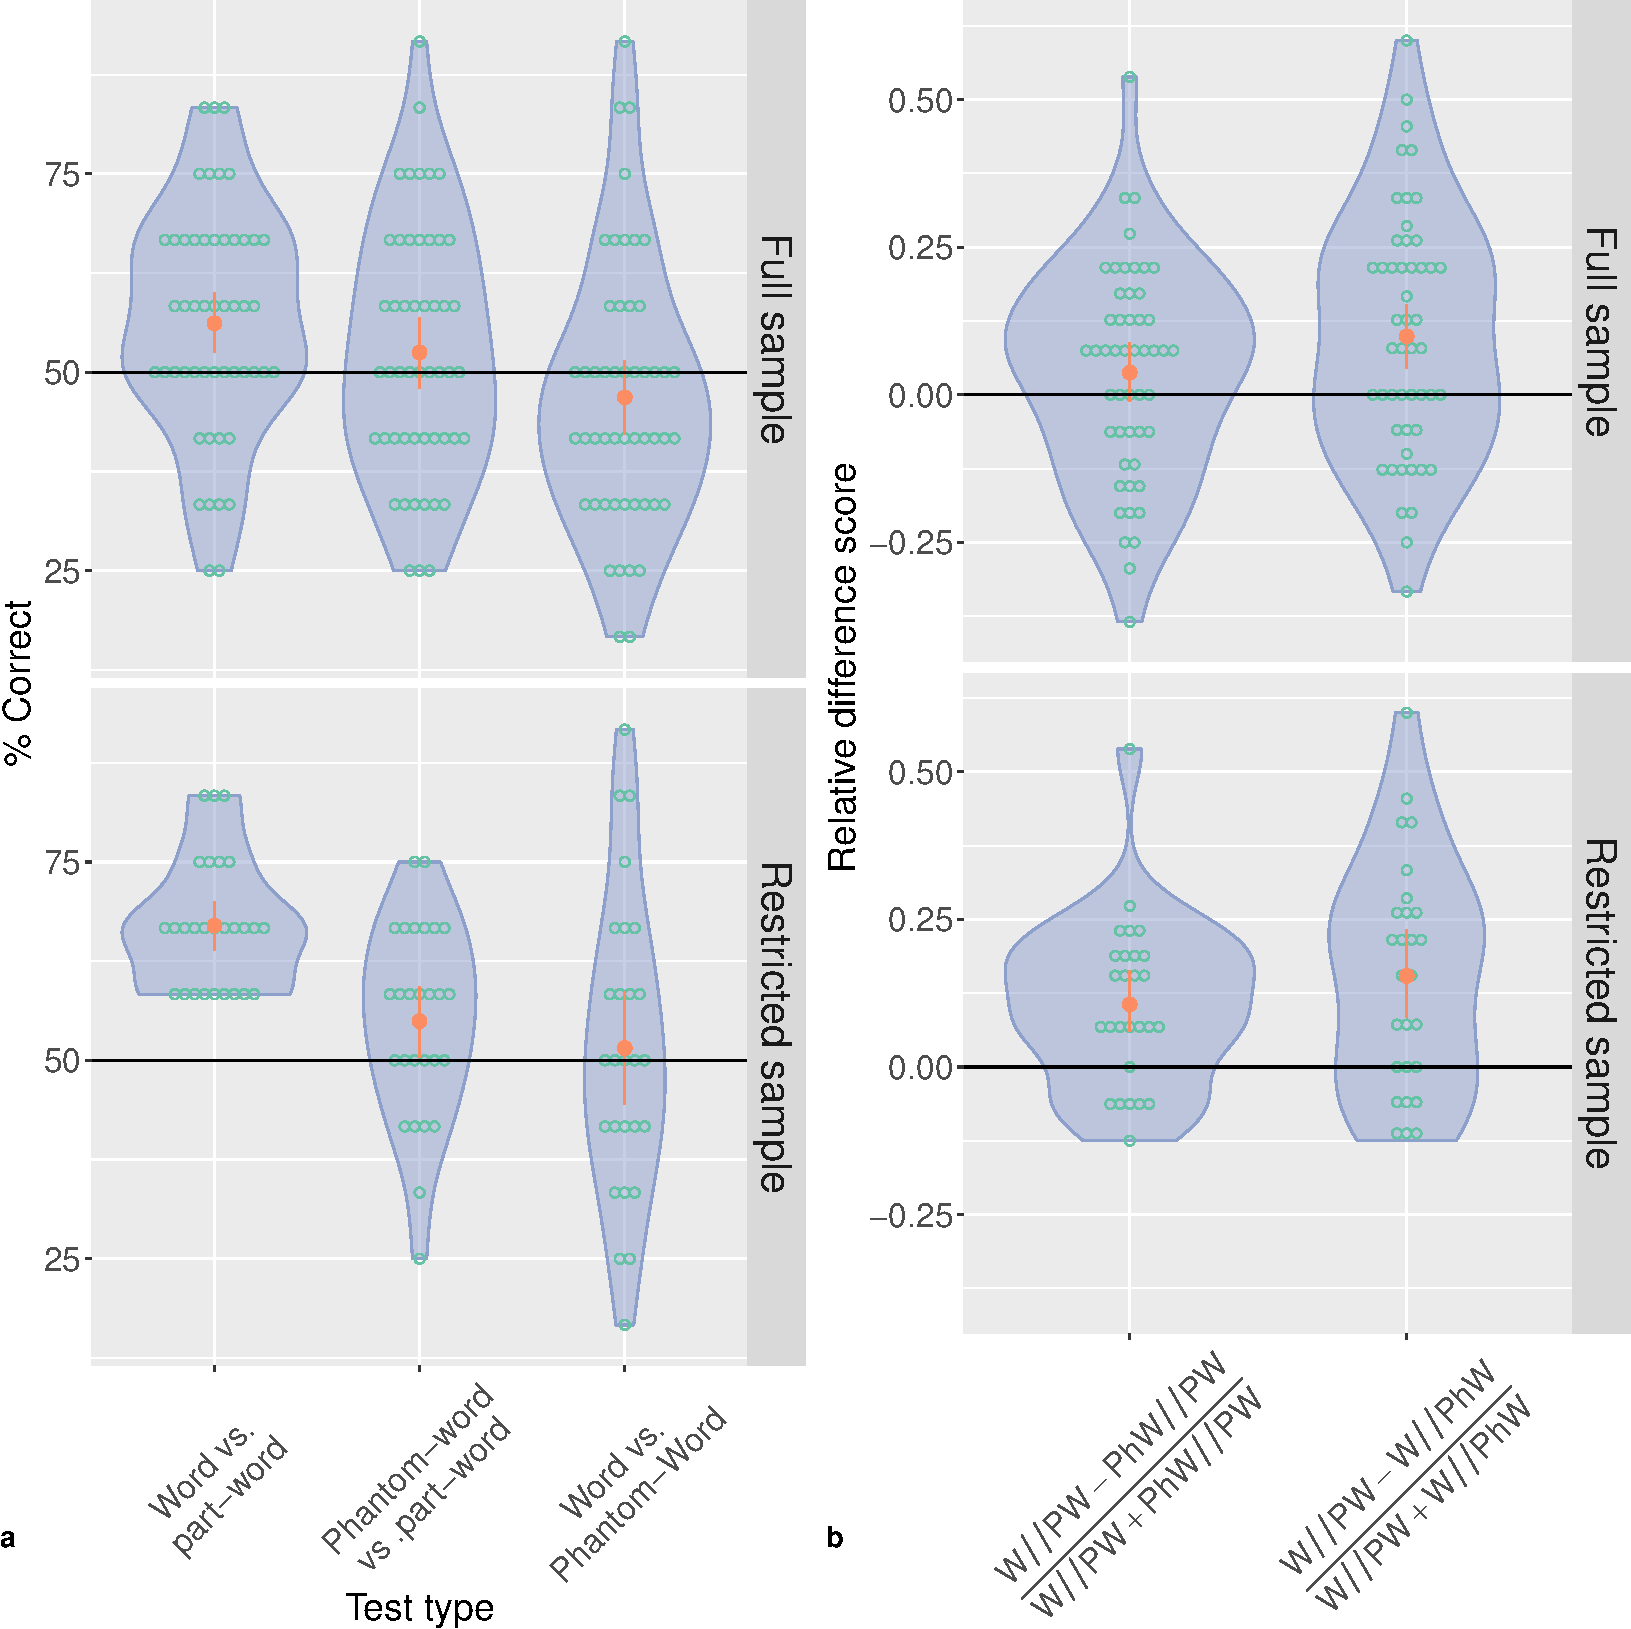
\includegraphics[width=0.8\linewidth]{vsl_phamtoms_simultaneous_results_files/figure-latex/vsl-simultaneous-fa-plot-accuracy-diff-scores-plot-polarity-collapsed-city-1} 

}

\caption{(a) Accuracy in the different trial types (words vs. part-words, phantom-words vs. part-words, and words vs. phantom-words), (b)  Relative difference scores for contrasts between different trial types (word vs. part-word trials vs. phantom-word vs. part-word trials, and word vs. part-word trials vs. word vs. phantom-word trials). Both panels show the data for the full student sample (top) or after exclusion of participants whose performance did not exceed 50\% in the word vs. part-word trials (bottom), collapsed across polarity contrasts (black shapes on a white background vs. white shapes on a black background). The dots, error bars and violin represent the sample averages, 95\% bootstrap confidence intervals and the distribution of the average accuracy for individual participants, respectively. Empty circles represent individual participants.}\label{fig:vsl-simultaneous-fa-plot-accuracy-diff-scores-plot-polarity-collapsed-city}
\end{figure}

\begin{figure}

{\centering 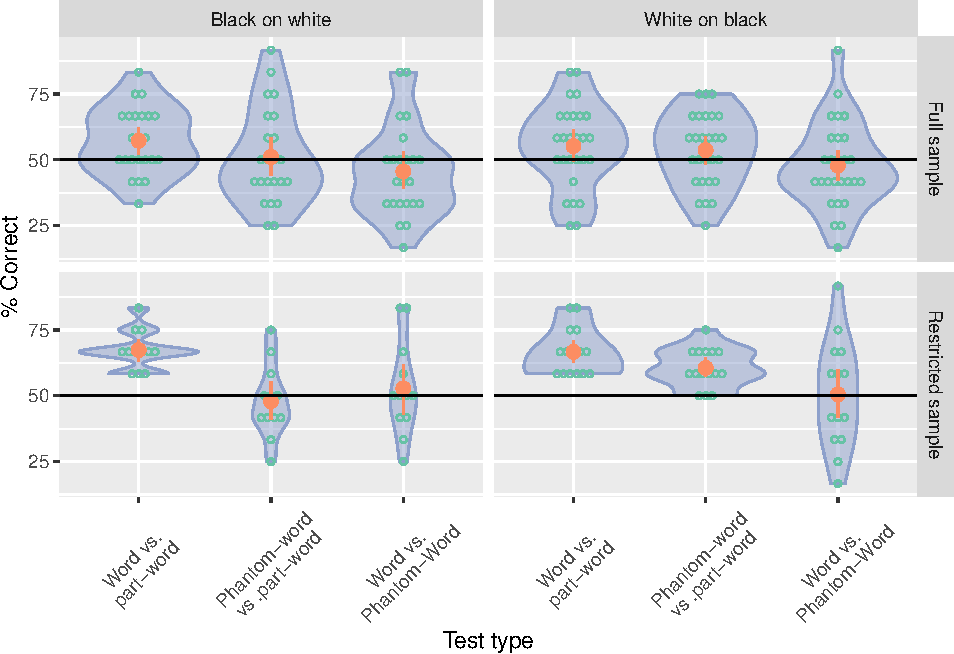
\includegraphics[width=0.8\linewidth]{vsl_phamtoms_simultaneous_results_files/figure-latex/vsl-simultaneous-fa-plot-accuracy-plot-by-polarity-city-1} 

}

\caption{Accuracy in the different trial types (words vs. part-words, phantom-words vs. part-words, and words vs. phantom-words), for the full student sample (top) or after exclusion of participants whose performance did not exceed 50\% in the word vs. part-word trials (bottom), for black shapes on a white background (left) and white shapes on a black background (right). The dots, error bars and violin represent the sample averages, 95\% bootstrap confidence intervals and the distribution of the average accuracy for individual participants, respectively. Empty circles represent individual participants.}\label{fig:vsl-simultaneous-fa-plot-accuracy-plot-by-polarity-city}
\end{figure}

\begin{figure}

{\centering 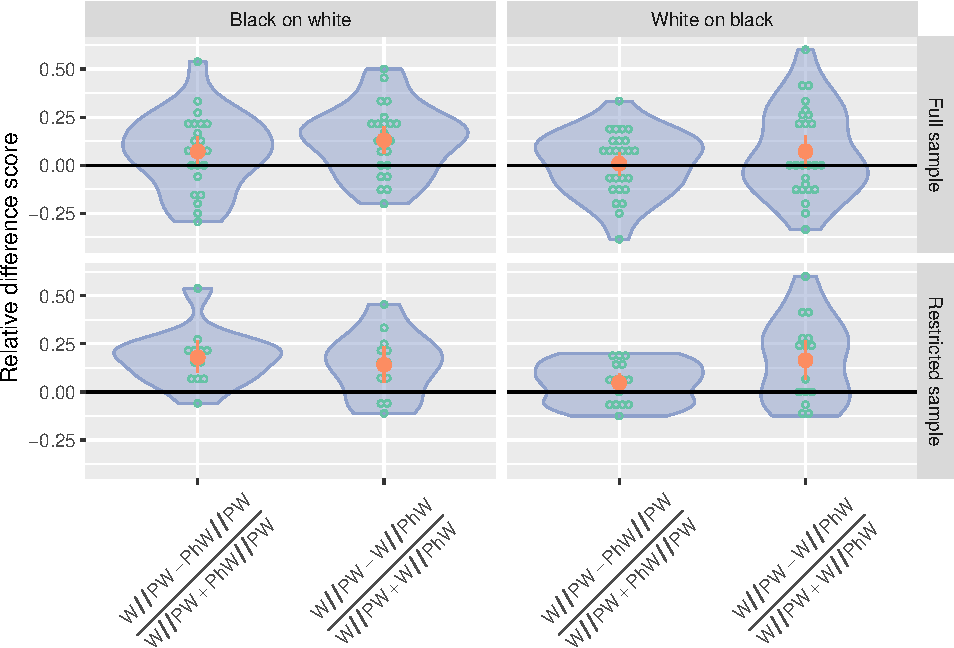
\includegraphics[width=0.8\linewidth]{vsl_phamtoms_simultaneous_results_files/figure-latex/vsl-simultaneous-fa-plot-difference-scores-plot-by-polarity-city-1} 

}

\caption{Relative difference scores for contrasts between different trial types (word vs. part-word trials vs. phantom-word vs. part-word trials, and word vs. part-word trials vs. word vs. phantom-word trials), for the full student sample or after exclusion of participants whose performance did not exceed 50\% in the word vs. part-word trials. The dots, error bars and violin represent the sample averages, 95\% bootstrap confidence intervals and the distribution of the difference scores for individual participants, respectively. Empty circles represent individual participants.}\label{fig:vsl-simultaneous-fa-plot-difference-scores-plot-by-polarity-city}
\end{figure}

The results for the student sample depended somewhat on whether the full
sample or the restricted sample were analyzed, and on whether a
correction for repeated testing was applied. This is presumably due to a
combination of the limited sample size, and the usually high proportion
of participants paying no attention to the stimuli.

The results for raw accuracy scores are given in Table
\ref{tab:vsl-simultaneous-fa-descriptives-print-city} and Figure
\ref{fig:vsl-simultaneous-fa-plot-accuracy-diff-scores-plot-polarity-collapsed-city}a.
(Individual results for the different polarity types are given in Figure
\ref{fig:vsl-simultaneous-fa-plot-accuracy-plot-by-polarity-city}.)

While participants in the restricted sample preferred words over
part-words (unsurprisingly, given that only those participants were
included who exceeded 50\% on the word vs.~part-word test), this
preference was only significant in the full sample when the
Holm-Bonferroni correction was not applied. In the restricted sample,
participants also preferred phantom-words to part-words, though this
preference survived the Holm-Bonferroni correction only when white
shapes were presented on a black background. In the full sample, this
preference was not significant. They had no preference for words over
phantom-words. There was no discernible effect of color polarity type.

To compare performance in the different trial types, I calculated the
difference scores mentioned above. As shown in Table
\ref{tab:vsl-simultaneous-fa-descriptives-print-city} and Figure
\ref{fig:vsl-simultaneous-fa-plot-accuracy-diff-scores-plot-polarity-collapsed-city}b,
participants from the student sample performed much better on word
vs.~part-word trials than on word vs.~phantom-word trials. While this
effect was generally significant before applying the Holm-Bonferroni
correction, it did not survive this correction for all polarity types.
Be that as it may, these results suggest that participants find
discriminations based on TPs much easier than discriminations based on
frequency of occurrence, which is problematic if statistical learning
leads to memory for units. (Individual results for the different
polarity types are given in
\ref{fig:vsl-simultaneous-fa-plot-difference-scores-plot-city}.)

However, at least in the restricted sample, performance was also
somewhat better for word vs.~part-word trials than for phantom-word
vs.~part-word trials, suggesting that we cannot rule out that
participants might also have some ability to track frequencies of
occurrence. However, the corresponding difference score was much smaller
than that comparing words vs.~part-word and word vs.~phantom-word
trials, and was not significant in the full sample.

\begin{longtable}[t]{lrrlrrlrrr}
\caption{\label{tab:vsl-simultaneous-fa-plot-glmer-correct-print-city}Results of generalized linear mixed models for trial-by-trial responses, for the student sample. Results are reported for the full sample as well as the restricted sample, where participants were excluded if their performance did not exceed 50\% on the word vs. part-word trials.}\\
\toprule
\multicolumn{1}{c}{ } & \multicolumn{3}{c}{Log-odds} & \multicolumn{3}{c}{Odd ratios} & \multicolumn{2}{c}{ } & \multicolumn{2}{c}{Power} \\
\cmidrule(l{3pt}r{3pt}){2-4} \cmidrule(l{3pt}r{3pt}){5-7} \cmidrule(l{3pt}r{3pt}){10-11}
term & Estimate & SE & CI & Estimate & SE & CI & t & p & power\\
\midrule
\addlinespace[0.3em]
\multicolumn{10}{l}{\textbf{Full sample - w.pw vs. w.phw}}\\
\hspace{1em}test.typew.pw & 0.475 & 0.173 & {}[0.136, 0.814] & 1.608 & 0.278 & {}[1.15, 2.26] & 2.743 & 0.006 & 0.800\\
\hspace{1em}color.typewhite.on.black & 0.090 & 0.183 & {}[-0.269, 0.448] & 1.094 & 0.200 & {}[0.764, 1.57] & 0.489 & 0.624 & 0.083\\
\hspace{1em}test.typew.pw:color.typewhite.on.black & -0.172 & 0.235 & {}[-0.633, 0.288] & 0.842 & 0.198 & {}[0.531, 1.33] & -0.733 & 0.463 & 0.097\\
\addlinespace[0.3em]
\multicolumn{10}{l}{\textbf{Full sample - w.pw vs. phw.pw}}\\
\hspace{1em}test.typew.pw & 0.251 & 0.172 & {}[-0.0862, 0.589] & 1.286 & 0.221 & {}[0.917, 1.8] & 1.460 & 0.144 & 0.299\\
\hspace{1em}color.typewhite.on.black & 0.106 & 0.176 & {}[-0.239, 0.452] & 1.112 & 0.196 & {}[0.787, 1.57] & 0.602 & 0.547 & 0.113\\
\hspace{1em}test.typew.pw:color.typewhite.on.black & -0.188 & 0.234 & {}[-0.647, 0.271] & 0.828 & 0.194 & {}[0.523, 1.31] & -0.804 & 0.421 & 0.140\\
\addlinespace[0.3em]
\multicolumn{10}{l}{\textbf{Restricted sample - w.pw vs. w.phw}}\\
\hspace{1em}test.typew.pw & 0.614 & 0.244 & {}[0.136, 1.09] & 1.848 & 0.451 & {}[1.15, 2.98] & 2.516 & 0.012 & 0.707\\
\hspace{1em}color.typewhite.on.black & -0.089 & 0.226 & {}[-0.532, 0.354] & 0.915 & 0.207 & {}[0.587, 1.42] & -0.394 & 0.693 & 0.061\\
\hspace{1em}test.typew.pw:color.typewhite.on.black & 0.058 & 0.327 & {}[-0.583, 0.698] & 1.059 & 0.346 & {}[0.558, 2.01] & 0.176 & 0.860 & 0.051\\
\addlinespace[0.3em]
\multicolumn{10}{l}{\textbf{Restricted sample - w.pw vs. phw.pw}}\\
\hspace{1em}test.typew.pw & 0.808 & 0.244 & {}[0.33, 1.29] & 2.243 & 0.547 & {}[1.39, 3.62] & 3.315 & 0.001 & 0.923\\
\hspace{1em}color.typewhite.on.black & 0.512 & 0.226 & {}[0.0691, 0.955] & 1.669 & 0.377 & {}[1.07, 2.6] & 2.266 & 0.023 & 0.649\\
\hspace{1em}test.typew.pw:color.typewhite.on.black & -0.543 & 0.328 & {}[-1.19, 0.0997] & 0.581 & 0.191 & {}[0.305, 1.1] & -1.656 & 0.098 & 0.387\\
\bottomrule
\end{longtable}

I confirmed these results using the generalized linear mixed models
above. As shown in Table
\ref{tab:vsl-simultaneous-fa-plot-glmer-correct-print-city}, the models
showed that performance on word vs.~part-word trials was significantly
better than for word vs.~phantom-word trials. They also showed that
performance on word vs.~part-word trials was significantly better than
on phantom-word vs.~part-word trials, though this predictor was
significant only in the restricted sample but not for the full sample.
In the model comparing word vs.~phantom-word trials and word
vs.~part-words and phantom-word vs.~part-word trials, performance was
somewhat better when white shapes were presented on a black background.
There were no other main effects or interactions with polarity type.

  \bibliography{/Users/endress/ansgar.bib}

\end{document}
